\section{Correlation, verification, and prioritization architecture}
Figure~\ref{fig:arch} shows the deployed computational order and Figure~\ref{fig:pipeline} provides a data-flow summary with alert counts. The correlation routine first groups same-source alerts, process-tree references, and eligible lineage references with host/account guards and a component-size cap of 100. It returns a partition and candidate diagnostics. Verification then inspects each visible relationship-token bundle before any additional cross-fragment union. Finally the ranking routine orders the resulting groups for the analyst. The repository's earlier code labels this as C--P--V in places, but the frozen prediction call executes correlation, then verification, then scoring; we describe this actual execution order as C/V/P.

\begin{figure}[ht]
\centering
\includegraphics[width=\linewidth]{fig2}
\caption{Detailed evidence-token bundle processing within the verifier. Each claim bundle is checked for provenance roots, temporal availability, and claim consistency. Only bundles that pass all three checks—and satisfy component-context guards—may add a cross-fragment union.}
\label{fig:corrarch}
\end{figure}

Verification outcomes in the implementation are reason-coded. A mismatched event or causal field, late claim, shared root, derived-only family, excessive component size, or incompatible component host/account context prevents union. An absent process claim may be considered by the constrained fallback in Section~\ref{sec:method}; its extra check uses receiver-visible endpoint fields, not truth labels. Rejected and insufficient proposals leave the existing partition intact. This is a conservative decision procedure under its assumed root semantics, not a formal guarantee against adversarially coordinated false observations.
\begin{figure}[ht]\centering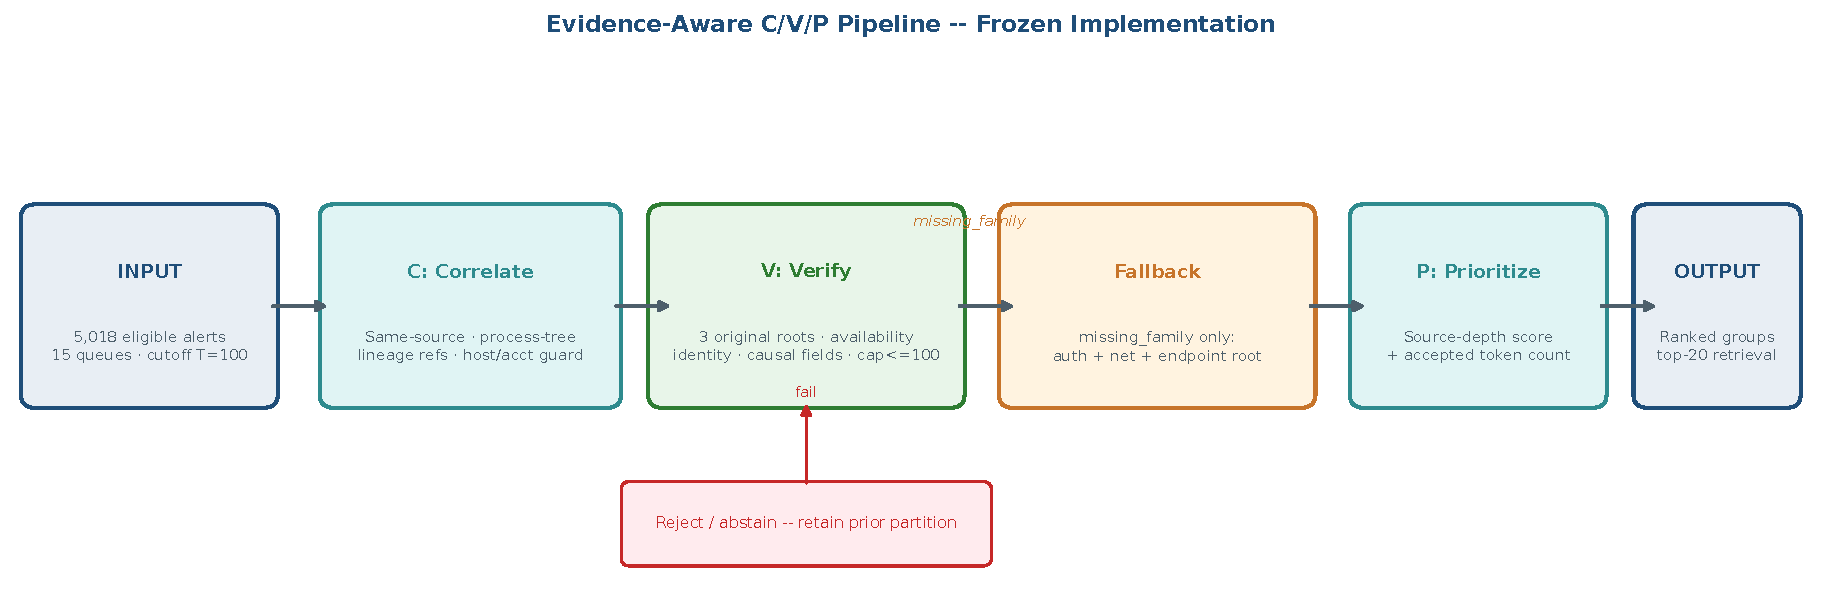
\includegraphics[width=\linewidth]{figures/pipeline_overview.pdf}\caption{Data-flow summary of the frozen C/V/P pipeline. The fallback branch is reachable only from the verifier for \texttt{missing\_family} rejections; all other failure modes retain the prior partition. Alert and queue counts are from the primary synthetic holdout (5,018 eligible alerts, 15 queues, cutoff $T=100$).}\label{fig:pipeline}\end{figure}
